


 \title{Third Week's Git Assignment} 

 \maketitle


\begin{abstract}
This document provide a brief introduction to Maximus' personal life, his goals, and his love for privacy.
\end{abstract}
\section{Background and Objectives for This Course}
Maximus a.k.a. \emph{"Cyber Gladiator"} works in the field of cybersecurity and is currently studying security this semester to focus on CPS/IoT designs, vulnerabilities, and flaws. As a student, he loves/ obsessed with privacy, and he hopes that he will become a more effective computer science researcher focusing on CPS/IoT systems by taking computer science research course this Fall.

Maximus' main area of interest includes (but not limited to) information systems’ vulnerabilities, vulnerabilities in system design and implementations, cyber risk assessment of IoT systems, and management of the risk in critical information systems in the broader context of their daily effects on individuals.


\begin{figure}[htbp]
\centerline{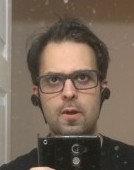
\includegraphics{a481.jpg}}
\caption{Maximus is currently looking at the mirror.}
\label{fig}
\end{figure}

Question 1: Have you focused any of your research in hardware vulnerabiilty specifically?  (from Cassandra Putman)  
<<<<<<< HEAD
=======

\textbf{Answer 1}: Great question Cassandra; and after I read your bio, I realized why you asked me this question.  Hardware security (and more broadly physical security) is one of the most important topics in IoT systems. Traditionally, security is more focused on protecting digital media in information systems; rather than focusing on physical security. In IoT, however, physical security can be more important because it can inflict real harm on people (and it will!). This is one of my areas of interest (to study of course) but couldn't find much literature by far. I am also thinking about researching in these areas. -Maximus
>>>>>>> 395e345b13e2f4e534ee67e0916c1dac96bbad64
